\chapter[需求不确定下的进口铁矿石多模式入厂物流网络优化]{需求不确定下的进口铁矿石多模式\\入厂物流网络优化}

尽管考虑中断风险的物流网络优化问题十分必要,但是中断风险发生的概率极低,需求的波动是一种常见的不确定来源,是决策者在进行短期决策时需要考虑的不确定因素。本章研究在需求不确定环境下钢铁公司进口铁矿石入厂物流网络优化决策问题。首先根据问题建立两阶段随机规划模型,然后根据问题结构设计基于拉格朗日情景分解的启发式算法,最后进行数值实验验证算法的有效性。

\section{问题描述}
\subsection{可持续生物燃料供应链优化研究综述}
生物燃料供应链的可持续性包括以下三个方面\cite{Awudu2012}:1)经济可持续性:涉及食物与能源、效率与能源之间的平衡问题以及生物燃料产业的预算问题等内容;2)环境可持续性:涉及减少碳排放、保护水资源、防止土壤退化、保护生物多样性等内容;3)社会可持续性:涉及促进就业、减少贫困、降低对士地作物的间接影响、降低对水资源等社会 公共资源的影响等内容。

针对生物燃料燃料供应链经济可持续性的研究相对多,主要侧重在对生物质生产、生物燃料生产、运输、库存等环节的经济可行性分析上。Kelloway等\cite{Kelloway2013}分别对以大豆和废弃食用油为原料的小规模生物柴油工厂进行技术一经济分析,结果表明以大豆为原料的小规模生产过程是不经济的, 而以废弃食用油为原料则是可行的。\citet{魏巧云2013}综合考虑生物质采购成本、运输成本和仓储成本,针对封闭式仓库干燥储存、半封闭结构棚无干燥储存和露天堆场无干燥储存三种储存方案的经济性进行比较。\citet{李璐2013}从不同主体之间的博弈关系出发,分析通过废弃食用油炼制生物柴油的原料回收成本和定价问题。一方面,该文献以“地沟油“非法生产作坊和生物柴油企业作为博弈主体,分析在有、无国家政策引导时的废弃食用油回收成本间题。结果表明,至少需要对非法作坊给予0.51倍的惩罚,才可以使生物柴油生产企业的原料采购成本下降。另一方面,该文献以废弃食用油回收企业和生物柴油生产企业作为博弈主体,分析两者应有的合理关系。结果表明,以生产企业为主、回收企业为辅的从属关系较两者的平等关系,更加有利于生物柴油产业的发展。Eijck等\cite{Eijck2014}针对2010-2030期间由5种生物燃料、8种生物质、12 个国家和8 种农业管理系统组成的74种一代/二代生物燃料供应链模式,分析供应链净现值和总生产成本,从而明确各类生物燃料的发展前景。结果表明,供应链投资回收期、投资规模和可选的产品市场取决于生物质种类,而生物质的选择取决千区域的农业系统、当地农户的偏好等。Correll等\cite{Correll2014}全面分析生物质采购、仓储、生产等成本,对比分析能源作物单一种植和多样化种植的经济效益。结果表明,当能源作物由单一种植方式转换为两种或三种混合种植方式时,将有助于减少2.38\%的物流成本。魏巧云\cite{魏巧云2014}以秸杆发电供应链为例,对比分析不同收集模式、运输模式和仓储模式的成本特性。王函\cite{王函2014}重点考虑运输成本、运输时间和运输线路长度三个因素,解决生物质的运输路线和车辆调度优化问题。

开展面向生物质供应、生物燃料生产和销售以及物流等环节的一体化供应链优化决策,从而实现经济指标最优,也是当前的主要研究方向之一。Parker等\cite{Parker2010}考虑农业废弃物、森林生物质、城市垃圾和能源作物四种生物质,结合美国西部现有的生物质来源、运输网络、生物燃料工厂和潜在的工厂节点等,建立以供应链利润最大化为目标的混合整数线性规划模型,解决工厂选址与定容、生产技术选择等问题。An等\cite{An2011a}质纤维素为原料的多周期、多产品的生物乙醇供应链作为研究对象,进行美国德克萨斯州中部地区的生物燃料供应链的设施选址与定容、技术选择、生物质分配等决策。Marvin等\cite{Marvin2012}面向大范围区域,针对以5种农业废弃物为原料的生物乙醇供应链, 建立以净现值最大化为目标的混合整数线性规划模型,并开展美国中西部9个州的案例研究。曹溢\cite{曹溢2013}将生物质电厂的选址问题分为两个阶段。第一阶段从原料供应维度、基础设施维度、政策环境维度和经济环境维度四个方面出发构建评价指标体系,并运用模糊综合评价法确定生物质电厂的可行选址方案栠合;第二阶段以物流成本最小化为目标,运用改进的重心法,从可行的选址方案集合中确定最优的选址方案。Shabani等\cite{Shabani2013}建立动态的非线性混合整数规划模型,针对以森林生物质为原料的发电厂,开展生物质采购、仓储、发电以及灰焊管理等多方面决策优化,从而实现供应链利润最大化。此外,将新型运输方式(如多式联运)引入生物燃料供应链之中也是当前的一个研究热点。Marufuzzaman等\cite{Marufuzzaman2014}研究多式联运设施连接具有一定中断概率时的生物燃料供应链优化。案例研究结果表明,当中断概率较低时,生物质运输将倾向于采用多式联运方式。Zhang等\cite{Zhang2016}考虑铁路与卡车运输两种方式,以总成本最小化为目标,进行设施选址与定容、原料和产成品的运输与库存等供应链决策。通过对美国密歇根州的案例研究,结果表明铁路运输在生物质长距离运输中发挥优势,而公路运输在短距离运输中发挥优势。

针对环境可持续性的考虑最初用于评估生物燃料产业的节能减排效果,如Ou等\cite{Ou2009}采用全生命周期法,对中国现有的六种生物燃料生产路径进行能源消耗和碳排放估算。这六种路径分别为以玉米提炼生物乙醇、以木薯提炼生物甲醇、以甜高粱提炼生物乙醇、以大豆提炼生物柴油、以麻疯树果提炼生物柴油和以废弃食用油提炼生物柴油。综合经济与环境性目标对生物燃料供应链开展一体化优化决策,成为近年的一个研究热点。Aldana\footnote{\label{ft:1}\bibentry{d_Amore_2016}} 等以能源产量最大化、成本最小化和碳排放量最小化为目标,建立混合整数规划模型,开展生物燃料生产技术选择(发酵和汽化技术)、工厂选址、客户选择等决策,并针对墨西哥以农业废弃物为原料的生物燃料供应链开展案例研究。Liu等\cite{Liu2014}运用生命周期法,综合考虑经济(年利润)、能源(能源消耗量)和环境性目标(碳排放量),首先对中国的生物燃料生产路径进行选择(包括生物乙醇、生物甲醇和生物柴油),其次开展生物质类型选择与种植选址、生物燃料生产设施选址以及供应链网络拓扑结构等一体化决策,最后对多目标开展帕累托最优分析。\citet{d_Amore_2016}考虑包含生物质种植与运输以及生物燃料生产、分配、使用等阶段的生物燃料全生命周期,以净现值最大化 和温室气体排放(包括对士地利用的影响)最小化为目标,解决多种生产技术时的供应链优化决策问题。然而单独地针对环境性目标开展供应链优化研究的文献很少,如Foo等\cite{Foo2013}以最小化运输环节的碳排放量为目标,对空果束的运输网络进行优化。

针对生物燃料供应链社会可持续性的研究主要集中千分析生物燃料产业对土地利用的直接和间接影响。第一代生物燃料导致的“与粮争地、与人争粮”问题,推动了学者们对生物燃料产业与农作物种植用地、粮食仗应安全之间关系的研究。Kristoufek等\cite{Kristoufek2012}采用最小生成树和层次树原理,分析衣副产品与生物燃料(生物柴冲、生物乙醇等) 之间的价格关系。通过对2007/2008世界根食危机发生之前和之后两个时期的数据进行对比,结果表明在粮食危机发生之后两 者的关系更为显著。Affuso等\cite{Affuso2013}\footnote{\bibentry{Affuso2013}}研究促进生物燃抖产业的土地可持续利用政策,提出了一种自愿性计划模型,并升展针对美国阿拉巴马川的仿真研究。结果表明,这种土地利用模式将分别增加高达215.68\%的生物燃料净能源值和减少高达19.67\%的碳排放呈,Oladosu等\cite{Oladosu2013}以美国2001-2010年的数据为基础,通运动态一般均衡模型仿真分祈生物燃料产业对土地利用的间接影响,Negash等\cite{Negash2013}通过对埃塞俄比亚农户的调杳发现,l)在供应链契约模式下,约1/3的农户倾向于将15\%的土地用于种植范麻,2)由契约带来的粮食产呈增长和农户收入增加,抵消了芭麻种杻对土地利用的影响,从而有助千提高农户的收入保障。此外,能源的供给安全也是社会可持续性的一个重要内容。Mansson等\cite{Mansson2014}研究瑞典玑有生物燃料(沼气、生物柴油和生物乙醇)的供应安全,并分析通过增加生物燃料产量和使用以实现能源安全和节能减拌目标的可能性。

\subsection{不确定条件下生物燃料供应链优化研究综述}
与其他产业相比,生物燃料产业具有更高的不确定性\cite{An2011}\footnote{\bibentry{An2011}}。部分文献已经开展了不确定条件下地区生物燃料供应链的发展前景评估研究。Hall等\cite{Hall2011}基于巴西的柔性燃科技术、大豆和蓖麻产量以及生物燃料的社会接受度等数据,分析技术、商业和社会三类不确定因素对生物燃料产业发展的具体影响。Zheng等\cite{Zheng2012}假设农民以利润最大化和风险规避为导向,研究在生物燃料产量和价格不确定条件下,农民的生物质种植意愿能否支撑起地区生物燃料产业的发展。通过美国华盛顿的案例研究表明,仅仅依靠华盛顿内部种植的生物匝,短期内难以满足区域生物燃料产业的发展需求。

面向单种或多种不确定因素,开展战略、战术、策略层面的优化决策是不确定条件下生物燃料供应链研究优化的主要方向。Awudu和Zhang\cite{Awudu2012}对2000-2010年期间的生物燃料供应链研究文献进行总结,提炼出生物页供给、物流、生物燃料生产、生物燃料需求与价格、政府税收与政策以及行业规范与政策等环节的不确定因素,并将不确定条件下的建模分析方法划分为数学分析方法(混合整数随机、线性规划、整数随机规划、混合整数随机非线性规划、情景式线性规划、马尔可夫决策过程)和数学仿真方法(离散事件仿真、蒙特卡洛仿真)两大类。

成本最小化、利润最大化、净现值最大化是不确定环境下生物燃料供应链优化研究中涉及最多的经济性目标。Chen等\cite{Chen2012}研究在生物质供应呈和生物燃料价格双重不确定因素的影响下,如何开展设施选址、生物质采购与运输以及生物燃料生产与销售等一系列决策,并建立以成本最小化为目标的混合整数随机规划模型。通过加拿大的实例研究表明,以废弃物生产生物燃料是经济有效的。Awudu和Zhang\cite{Awudu2013}考虑由生物质供应商、生物燃料精炼工厂和配送中心组成的三级供应链结构,分别以已知随机分布函数和几何布朗运动分布函数描述生物燃料市场需求和价格的不确定性,并据此建立以利润最大化为目标的生产计划随机规划模型。研究结果表明,采用随机规划模型较不考虑不确定因素的确定性规划模型取得更高的期望收入。Azadeh等\cite{Azadeh2014}提出多周期的随机线性规划模型,通过设施选址、原料生产、运输分配、生产技术选择以及库存等决策优化,从而实现利 润最大化,并采用敏感性分析法刻画生物燃料需求和价格变化对供应链利润的影响机理。Giarola等\cite{Giarola2012}提出一个动态的、直观的、多级的混合整数线性规划模型构建框架,解决在生物质和生物燃料价格不确定条件下,如何合理安排工厂位置、原料和产品分配计划,以最大化供应链净现值。

也有少量研究以经济风险性作为优化目标。Shabani等\cite{Shabani2014}按月估算生物质的供给不确定性,并以供应链利润最大化和不确定风险(可变性指标、下跌风险)最小化为目标,建立两阶段的多周期随机规划模犁,从而开展生物质采购、仓储和发电决策。案例研究结果表明,生物质电厂需要为原料供给不确定性支付40万美元/年的额外费用,但采用随机规划模型可以将这一费用降至20万美元/年。Babazadeh等\cite{Babazadeh2017}采用“井口到车轮” 作为生物柴油的生命周期阶段,并将供应链成本、碳排放量和风险作为优化目标,提出随机规划模型和帕累托最优求解算法。针对伊朗的案例研究结果表明,供应链决策者需 要在经济、环境和风险目标之间进行良好的权衡。

设施选址与定容决策属千战略层面,而生物质和生物燃料的物流问题属千战术或运营层面。因此不少研究采用两阶段规划方法,对战略、战术或运营层面的决策进行区分。 一般而言,两阶段规划的第一阶段解决涉事选址与定容问题,而第二阶段问题解决原料与产品的物流计划问题。Kim等\cite{Kim2011}采用不同情景描述生物质产量以及生物燃料生产技术、需求、价格不确定性,建立以利润最大化为目标的两阶段混合整数随机规划模型。Osmani等\cite{Osmani2013}以柳枝稷和农业废弃物两种生物质为原料,考虑在柳枝稷产量、农业废弃物价格、生物乙醇需求和价格不确定条件下,建立两阶段随机规划模型,解决工厂选址、生物质采购和运输、生物燃料生产与销售等问题。针对美国北达科他州的研究案例表明,伴随着供应链不确定程度的增加,供应链的经济效益将有所下降,但生物燃料工厂的选址决策受不确定性的影响程度并不高。Li和Hu\cite{Li2014}考虑由小型快速热解厂和大型生物燃料精炼中心组成的分布式网络,解决原料供给、生物燃料生产技术与价格不确定条件下的设施选址与定容、生物质和生物燃料的物流问题。

与确定条件下的生物燃料供应链优化模型类似,开展不确定条件下生物燃料供应链的环境影响评估同样受到了国内外学者们的关注。Giarola等\cite{Giarola2012}同时考虑生物质供给不确定性和碳排放配额交易计划,以供应链净现值最大化和碳排放最小化为目标,建立多周期、多层次的混合整数线性规划模型,从而解决生物乙醇上游供应链的原料分配、生产技术选择以及工厂选址等问题。黎玉婷\cite{黎玉婷2013}结合需求不确定性,分别考虑强制排放和碳税两种政策,对比分析露天堆场无干燥储存和封闭式仓库干燥储存两种生物质库存策略的经济效益。Osmani和Zhang\cite{Osmani2014}以利润最大化和碳排放量最小化为目标,针对生物质供给、生物燃料需求与价格不确定条件,建立两阶段随机规划模型,并面向美国中西部4个州中以木质纤维为原料的生物燃料供应链开展案例研究。

生物燃料供应链是一种较为特殊的供应链,它的上游农场废弃物(或城市废弃物)回收供应链交叉,而下游戏与石油供应链重叠。因此,一些研究开始将生物燃料供应链与废弃物回收供应链或石油供应链进行结合。Tong等\cite{Tong2014}将生物燃料供应链与现有的石油供应链进行结合,提出原料共同处理、生产设施混合和最终产品混合三种结合策略,针对生物质供给与转化率、生物燃料生产成本以及生物燃料工厂设施成本等多种不确定条件,建立以成本最小化为目标的多周期混合整数规划模型,进而开展设施选址、生物质种植、生产技术选择、生物燃料生产和销售等决策,并对美国的伊利诺斯州开展案例研究。Yeh等\cite{Yeh2015}将生物燃料供应链与现有的林场供应链进行结合,以林场的种植者(决定生物质收获数呈)和生物燃料生产者(决定生物燃料产量)作为两个博弈对象,解决生物质供给水平与价格以及生物燃料生产成本、市场需求、未来价值等多因素不确定条件下的设施选址与定容、供应链决策者的博弈关系等问题。

基于上述的不确定条件下生物燃料供应链优化文献,本文得出以下几点重要结论。

•生物燃料供应链的不确定性涵盖生物质供给、生物燃料生产与销售、政府政策与行业规范以及物流等多个方面,但生物质供给(价格、供给水平等)和生物燃料需求(价格、需求水平等)不确定性是最受关注的。

•不确定条件下生物燃料供应链的决策内容主要包括设施选址与定容、生物质与生物燃料的运输计划、库存决策以及生产技术选择等。

•生物燃料供应链优化目标包括经济性目标(成本、利润、净现值等)、环境性目标(碳排放、能源消耗等)和社会性目标(对士地利用的影响、对社会公共资源的影响等)。当前文献中对经济、环境性目标的研究较多,但尚无文献综合经济、环境和社会三个方面开展生物燃料供应链可持续优化的研究。

•不确定条件下生物燃料供应链优化的方法主要集中于情景式规划、随机规划等,而很少有文献开展生物燃料供应链鲁棒优化的相关研究。

\subsection{生物燃料供应链鲁棒优化研究综述}
将鲁棒优化理论应用干生物燃料供应链优化的相关研究当前还较为缺乏。Foo等\cite{Foo2013}从电热联产企业角度出发,分别构建鲁棒线性规划模型和鲁棒混合整数规划模型,进而解决生物质供给不确定条件下的生物燃料生产设施选址和原料分配问题。Tong等\cite{Tong2014a}采用不同清景描述生物质供给和生物燃料需求不确定性,将现有的加油设施纳入供应链优化之中,进而构建起一体化供应链决策的鲁棒优化模型,并设计相应算法解决鲁棒约束和经济性目标之间的权衡问题。Shabani和Sowlat\cite{Shabani2016}研究生物质含水董不确定性对生物质电厂经济效益的影响,提出多周期的随机鲁棒优化混合模型,解决生物质电厂的原料分配和库存管理问题。案例研究结果表明,当生物质的含水星和热值分别在$\pm13\%$和$\pm5\%$波动时,生物质电厂的利润下降最高可达$23\%$。

目前,尚无文献将可持续目标(同时包括经济、环境和社会三个方面)理论同时应用于生物燃料供应链优化之中。生物燃料供应链的发展必定要满足经济、环境、社会等多方面的可持续发展,而且也需要应对来自供应链自身和外界环境的各类不确定因素,从而提升生物燃料的市场竞争力。因此,针对当前文献中对千生物燃料供应链鲁棒性和可持续目标考虑的缺乏,本文着眼千不确定条件下可持续生物燃料供应链舍棒优化问题,将经济、环境、社会等可持续目标和鲁棒优化理论同时引入生物燃料供应链优化之中。

\section{生物燃料供应链的组成与决策内容}

\subsection{生物燃料供应链组成}

生物燃料供应链的利益相关主体包括生物质供应商、生物燃料生产商、生物燃料消费者、物流企业以及政府和行业监管机构\cite{Seay2014}。因此,一个完整的生物燃料供应链至少需要包括以下几个组成部分:来自单个或多个区域的生物质供应商、一个或多个生物质和生物燃料仓储设施、一个或多个生物燃料精炼工厂、一个或多个阶段进行预处理操作的设施以及一种或多种运输方式的设施节点\cite{Shabani2013},如\figref{fig:biofuelsc}所示。
\begin{figure}[htbp]
	\centering
	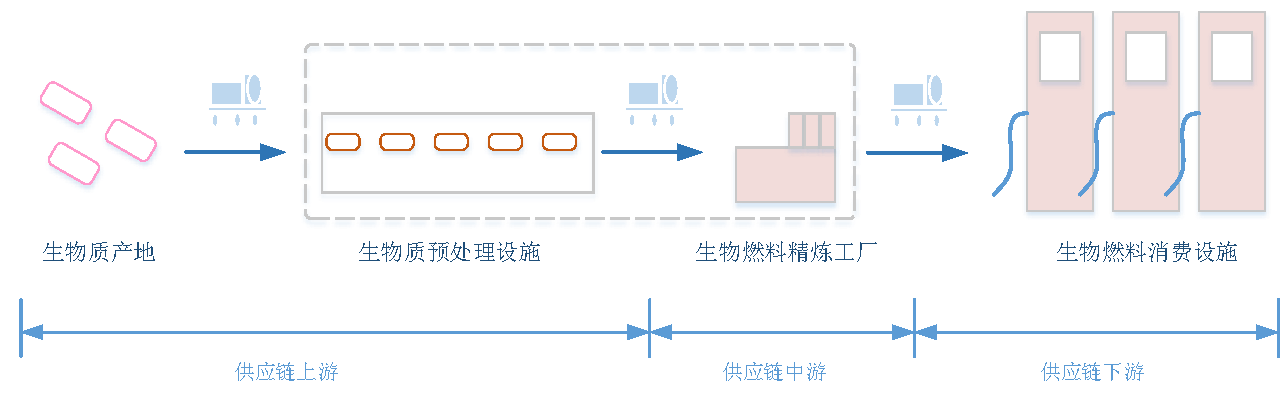
\includegraphics[width=\linewidth]{biofuelsc.pdf}
		\setlength{\abovecaptionskip}{0pt}%

	\setlength{\belowcaptionskip}{0pt}%
	\caption{生物燃料供应链示意图}

	\label{fig:biofuelsc}
\end{figure}

图中所示的各个组成部分具体为:

\begin{compactitem}
	\item 生物质产地:生物质包括所有的植物和植物衍生的材料(包括但不局限千糖类、油类作物)以及动物脂肪等\cite{An2011}。生物质的产地分布与生物质种类密切相关, 如秸杆、玉米棒等农业废弃物属千衣作物收割后的残留物,一般集中分布千衣场附近;废弃食用油主要混合于城市餐厨垃圾之中,因而零散分布千城市的餐饮企业、宾馆以及居民生活区等。
	
	\item 生物质预处理设施:预处理的目的在千提取生物质中可用于转化为生物燃料的部分或成分,从而保证生物燃料的顺利生产,并在长距离运输中发挥着降低运输成本的作用。对于农业废弃物而言,预处理工作包括干燥、切片、包装等步骤\cite{Gold2011},从而降低生物质的含水量,进而提高运输过程中装卸、搬运的方便性。
	
	\item 生物燃料精炼工厂:生物燃料精炼工厂是将生物质转化为生物燃料的设施。
	
	\item 生物质和生物燃料仓储设施:生物燃料的仓储条件与汽油、柴油等类似,因此本文着重阐述生物质的仓储过程。一般而言,生物质存在分散仓储和集中仓储两种模式。以农业废弃物为例,前者利用农户周边的空地等作为仓储设施,因而成本相对较低,但也给衣户造成了一定的库存积压,并引发生物质的仓储条件不统一、损耗严重等问题;后者由生物质收集者将生物质统一收购后再进行集中存储,可以保证较好的仓储条件,从而减少原料损耗,但相应的成本也较高。
	
	\item 运输设施节点;对千衣业废弃物而言,生物质一般位于较为偏僻的衣村,与生物燃料主要消费地(城市)之间存在一定的空间距离。而生物燃料工厂既可以设置为靠近衣场(靠近供给点),也可以设置为靠近城市(靠近消费点), 或者是在两者的中间。因此,生物燃料供应链运作过程中必然存在原料和产品运输距离的权衡问题。在实际运作中一般考虑在保证各种运输方式可达性的基础上,选择成本最低的运输方式。这既可以是单一的运输方式(一般为道路运输),也可以是多种运输方式的联运。
\end{compactitem}

\subsection{生物燃料供应链典型结构}
生物燃料供应链的具体结构与原料种类、原料分布、采用的生产技术、运输方式以及产品用途都存在一定的关系。生物质种类较为繁多,其地理分布也存在千差万别,因而很难从原料种类和分布情况的角度,给出一个统一的供应链结构。因此,本文重点从生物燃料生产策略的角度对供应链结构进行阐述。一般而言,生物燃料的生产策略分为集中和分散两种策略\cite{Liu2014}。其中,集中策略将生物质直接由供给点运送到生物燃料工厂,并转化为生物燃料;分散策略将生物质先运送到距离供给点较近的第一级小型工厂(生物质预处理设施)并转化为中间产品,随后再将中间产品运送到大型工厂并统一转化为生物燃料。

与生产策略相对应,生物燃料供应链主要包括两种基本结构。对千集中策略而言,生物质直接运送至生物燃料工厂,因而生物质的预处理和转化作业是在同一地点完成的。因此,该供应链的基本结构应该为“生物质供给点—一体化生物燃料精炼工厂—生物燃料消费地” 组成的三级结构(\figref{fig:biofuelsc}虚框为一体化生物燃料精炼工厂)。而对千分散策略而言,生物质优先转化为中间产品,再棠中转化为生物燃料,因而生物质的预处理 和转化作业是在不同地点完成的。因此,该供应链的基本结构应该为“生物质供给点—生物质预处理设施—生物燃料精炼工厂—一生物燃料消费地”组成的四级结构。

\subsection{生物燃料供应链决策内容}
供应链优化是生物燃料可持续生产的一个的重大挑战\cite{Seay2014}。它在空间尺度上涉及生物质生产到生物燃料消费的整个过程,在时间尺度上涉及单元操作到生物燃料生产的整个价值链,具体包含如何在战略层面、策略层面和运营层面实现成本效益、系统鲁棒性和可持续性\cite{Yue2014}。供应链的运行效率则取决于生物质的地理分布、生物燃料的生产作业以及燃料市场的准入成本等多方面因素\cite{Chen2012}。这些因素不是相互独立的,它们相互影响、相互作用, 共同反映出生物燃料供应链的整体运作效率\cite{Bai2012}。

如\tblref{tbl:content}所示,生物燃料供应链的优化决策应该从战略、策略和运营三个层面出发\cite{Awudu2012,An2011,Meyer2012}:

•战略层面:解决长期(年度或更长时间段)的决策,具体包括:1)生物质的种植与采购策略;2)生物燃料的生产策略;3)生物燃料供应链的设施建设策略;4)原料与产品的物流网络优化与模式选择;5)长期需求契约设计。

•策略层面:解决较长时期(月度或季度)的决策,具体包括:1)生物质的收获时间与数量计划;2)原料和产品的物流车辆调度与库存决策;3)生物质燃料的生产计划与需求预测。

•运营层面:解决短期内(每小时、每日或每周)的决策,具体包括:l)日常车辆调度与日常库存管理;2)生物燃料的日常生产计划。

\begin{table}[htbp]
	\centerfloat
	\zihao{5}
	\caption{生物燃料供应链优化决策内容}\label{tbl:content}
	\begin{tabular}{>{\centering}p{60pt}>{\centering}p{150pt}p{200pt}}
		\toprule
		决策层面 & 决策内容 & 具体内容\\
		\midrule
		\multirow{9}{*}{战略层面}&生物质供给策略&生物质类型、生物质种植技术、生物质种植土地面积、生物质供应商、生物质供应地点、生物质供应契约\\
		\cmidrule{2-3}
		&生物燃料生产策略&生物燃料生产技术\\
		\cmidrule{2-3}
		&供应链设施建设建议策略&预处理设施选址与定容、生物燃料工厂选址与定容、仓储设施选址与定容\\
		\cmidrule{2-3}
		&原料与产品物流策略&分散或集中库存模式、运输模式选择、运输网络涉及、物资分配\\
		\cmidrule{2-3}
		&生物燃料需求策略&生物燃料需求契约\\
		\midrule
		
		\multirow{5}{*}{策略层面}&生物质收集策略&生物质收集时间、收集数量\\
		\cmidrule{2-3}
		&生物燃料生产策略&生物燃料产量\\
		\cmidrule{2-3}
		&生物燃料需求策略&需求预测和审查\\
		\cmidrule{2-3}
		&原料与产品物流策略&库存策略、运输工具选择、运输路线设计、运输车辆调度、物流合同\\
		\midrule
		
		\multirow{2}{*}{运营层面}&原料与产品物流策略&日常库存策略、运输车辆调度\\
		\cmidrule{2-3}
		&生物燃料生产策略&工厂生产计划、物料需求计划\\
		
		\bottomrule
		
	\end{tabular}
\end{table}

\section{生物燃料供应链的可持续性}
\subsection{生物燃料供应链可持续性内涵}
能源可持续性意味着既满足当代人为实现环境管理、经济繁荣和生活质量提升的能源需求,又不损害后代人满足这些需求的能力。当前可持续供应链设计已经成为一种新兴方法,它尝试在供应链设计中涵盖经济、环境以及社会的相关决策\cite{Chaabane2012}。这也就是说,经济、环境和社会指标成为衡鱼供应链可持续性的三个重要标准\cite{Meyer2012}。

生物燃料作为一种石油、汽油等传统燃料的新兴替代能源,而如何保证产品的价格竞争力和连续生产供应,对千生物燃料产业的发展至关重要\cite{Gold2011}。其中需要重点关注的是,如何从经济效益、能源消耗以及环境影响等可持续性出发,保证整个过程的可行性。总之,生物燃料供应链的可持续性内涵应该包括经济方面、环境方面和社会方面,具体表现为\cite{Awudu2012,An2011,Meyer2012,Zonin2014}:

•经济方面:主要强调如何保障社会、产业以及供应链等层面的经济可行性,具体包括:l)食物与能源的争论问题;2)效率与能源之间的平衡问题;3) 生物燃料产业的预算问题;4)供应链运作成本与利润优化问题;5)供应链现值评估问题;6)投资风险规避问题。

•环境方面:主要强调如何减少对土地资源、水资源、能源的消耗,降低碳排放、污染物排放等环境影响,具体包括:1)碳排放以及对全球气候变暖的影响问题;2)水资源的利用问题;3)士壤健康问题;4)生物多样性问题;5)能源回报率问题;6)空气污染的控制问题;7)水体污染的控制问题;8)废弃物的监管问题;9)化肥的合理使用问题。

•社会方面:主要强调如何提升社会福利、推动就业等方面,具体包括:1)促进就业间题;2)减少贫困问题;3)对土地作物的间接影响问题;4)对水资源等社会公共资源的影响问题;5)产品责任问题;6)保障公众健康问题;7)食品安全问题;8)与法律法规的符合程度问题;9)文化接受程度问题;10)噪声影响问题。

\subsection{生物燃料供应链经济可持续性衡量方法}
生物燃料供应链的可待续性可以从经济、环境和社会三个层面进行分析, 而每个层面又涉及到多个子指标。这些指标又可以分为定量和定性两类指标。但结合供应链优化过程的指标定噩化需求, 本文重点阐述常用的定量指标衡量方法。

\subsubsection{供应链成本}
第二代生物燃料在节能减排效果、土地利用影响等方面都比第一代生物燃料有了较大的改善,但其生产成本仍然较高,与汽油、柴油等化石燃料相比缺乏价格竞争力,进而严重限制了生物燃料的产业化进程\cite{Giarola2012}。因此从供应链优化角度出发,协调生物质采购、生物燃料生产与销售以及物流等一系列环节,降低供应链成本已经成为当前研究的重中之重。\figref{fig:biofuelcost}展示了生物燃料供应链各个环节的主要成本构成。本文将逐一进行详细说明。

\begin{figure}[!htbp]
	\centering
	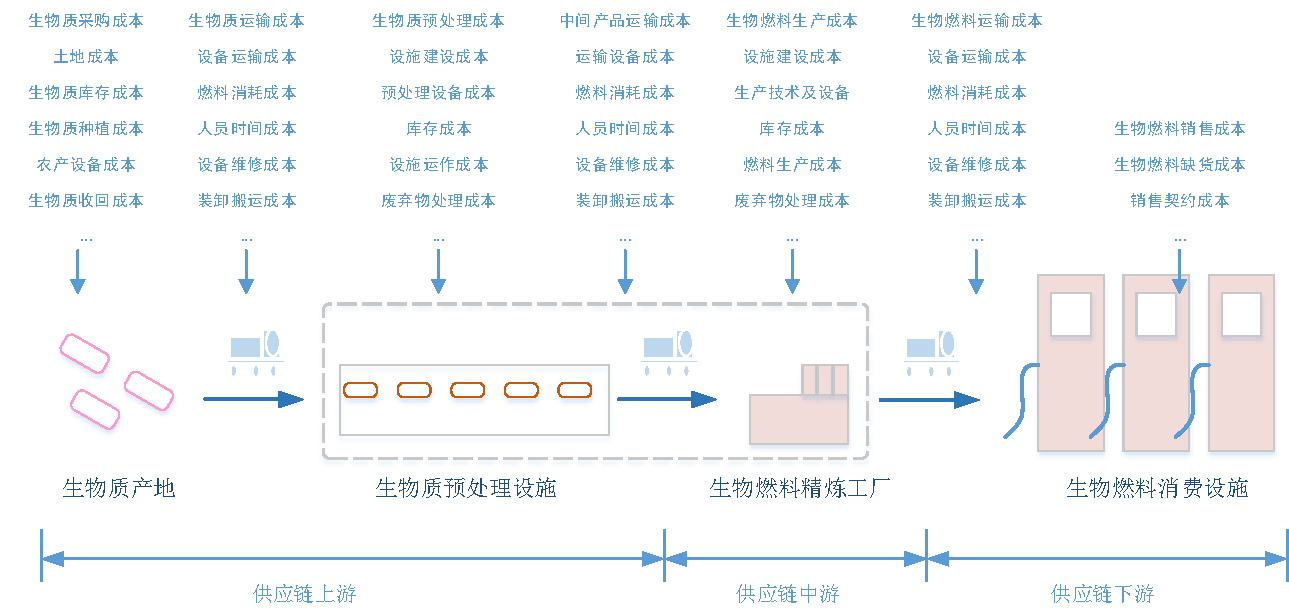
\includegraphics[width=\linewidth]{biofuelcost.pdf}
	\caption{生物燃料供应链的主要成本构成}
	\label{fig:biofuelcost}
\end{figure}

(1)生物质种植与采购环节

生物质种植环节的成本主要包括土地使用成本,人力、化肥等相关投入以及生物质收获成本等\cite{Osmani2013}。这些成本由衣户(生物质种植者)进行支付,并最终反映到工厂的生物质采购成本上。对于工厂而言,生物质的采购分为长期契约采购和临时采购两种方式\cite{Correll2014}。长期契约采购方式指生物质采购商(工厂或其他中间商)与供应商签订长期契约合同(数量折扣契约、收益共享契约等),从而获取相对低廉的采购价格。长期契约采购方式尽管带来相对低廉的采购价格,但在实际运作中受供应商违约、生物燃料市场需求波动等因素影响,可能导致工厂出现生物质供应不足的现象。此时,工厂需要采用成本相对较高的临时采购方式,即从外部市场临时购入生物质以补充原料供应。因此在供应链优化建模中,生物质采购成本的衡量需要根据采购的方式而定,既可以表示为契约采购成本,也可以表示为临时采购成本,或是两者皆有。其中,临时采购一般以采购数量与采购价格的乘积进行估算\cite{Chen2012},而契约采购与前者的不同之处在于采购价格可能与采购数噩或者其他因素相关。

(2)生物质预处理环节

预处理环节的成本包括设施建设成本、设备购置成本等固定成本以及生物质预处理成本、生物质预处理前后的库存成本、废弃物的处理成本等可变成本。固定成本一般通过一定的折旧年限进行分摊,而可变成本则通过需要预处理的原料数量和单位成本的乘积进行估算\cite{Chaabane2012}。

(3)生物燃料生产环节

生产环节的成本包括设施建设成本、生产设备购置成本(生产技术投入成本)等固定成本以及生物燃料生产成本、库存成本、废弃物处理成本等可变成本\cite{Jiang2014}。生产设施的建设成本不仅与设施所处的位置、采用的生产技术有关,而且与设施的规模密切相关。因此,建设成本的衡量应该包括与规模无关的固定部分和与规模相关的可变部分\cite{Chen2012,Sabio2012}。可变成本则主要与生物燃料的产量挂钩。而且当生产设备容堡不足以满足生产需求时,工厂可能需要采用生产外包方式,由此产生生产外包成本\cite{Akgul2012}。

(4)生物燃料销售环节

销售环节是供应链产生利润的环节,但也需要支付产品宣传、销售场地租赁、合同签订等销售费用。这些费用相对比较固定,且占据销售收入的比例不大,一般不纳入供应链优化建模之中。此外,生物燃料销售商需要保证一定的服务水平。因此,由千产品缺货而导致的缺货成本也是销售环节成本的一个重要组成部分\cite{Osmani2013}\cite{Li2014}。一般而言,缺货成本是通过未满足的需求数量与单位缺货成本的乘积进行估算。

(5)供应链物流环节

物流环节对供应链成本有着显著的影响”叽运输和仓储是物流的两个重要功能,也是物流成本的两个主要组成部分。对千运输环节而言,其相关成本包括运输设施建设、运输设备购置等固定成本以及运输过程中产生的可变成本。固定成本的计算相对简单,一般通过一定的折旧年限进行分摊,而可变成本与运输货种、运输方式等多因素相关,计算相对复杂。从运输货种上看,生物燃料供应链主要包括生物质、经过预处理的生物质(中间产品)和生物燃料三类货种。因此,供应链建模中需要分别计算这些货种的运输成本\cite{Chaabane2012}。从运输方式上看,上述货种既可以采用单一的运输方式,也可以采用多种运输方式开展多式联运。因此,运输成本的计算还需要结合具体的运输方式。对千单一的运输方式而言,运输成本一般通过运输距离、运输量与单位运输成本的乘积进行估算,而单位运输成本又包含车辆油耗成本、装卸成本以及驾驶员工作时间成本等\cite{Chen2012}。对于多式联运而言,除了需要估算各种运输方式的相关成本之外\cite{Sabio2012}, 还需要估算运输方式之间的转运成本以及集装箱运输下的空箱调度成本\cite{Marufuzzaman2014}。

与运输环节类似,仓储环节的成本估算也需要分货种进行。库存成本不仅与库存条件(影响单位库存成本)、库存水平密切相关,而且与库存策略(如供应商分散库存和工厂集中库存)相关。在供应链建模中,库存成本一般通过平均库存水平与单位库存成本的乘积进行估算\cite{Correll2014}。

\subsubsection{供应链利润}
利润是生物燃料产业盈利情况的直观反映,也是供应链成员经营的最主要目标和直 接激励。供应链利润为供应链收入与成本的差值\cite{Li2014}。由千前文已经对供应链成本进行了详细的阐述,本文在此重点分析供应链的收入估算方法。生物燃料供应链的收入来源主要包括以下几个方面:1)生物燃料销售收入:生物燃料需求存在固定和非固定需求两种类型,对应的销售方式也分为契约销售和临时销售两种方式\cite{Shabani2014}。两种销售方式的主要区别在千销售数昼和价格的不同,但销售收入均为销售数呈与销售价格的乘积。2)副产品销售收入:生物质在转化为生物燃料之后,将产生诸如酒糟、化肥原料等副产品。这些 副产品既可以直接销售,也可以由生物燃料工厂进一步加工成其他产品后再销售\cite{Balaman2014}。3)政府补贴:生物燃料作为化石燃料的替代能源之一,得到世界各国政府的大力支持。补贴或税收减免是政府经济性激励的常用措施,从而给供应链带来一定的收入\cite{Osmani2013,Osmani2014}。

\subsubsection{供应链净现值}
供应链净现值指生物燃料供应链的预期收入现值与成本现值的差额。净现值本质上也是基千供应链收入和成本进行估算\cite{Marvin2012,Giarola2012,Giarola2012,Sabio2012,Zamboni2011},涉及的指标也均与前文阐述的类似。供应链净现值与利润的主要不同点在于,净现值需要通过折现率将预期收入和预期成本转化为现值。

\subsection{生物燃料供应链环境可持续性衡量方法}
生物燃料供应链环境可持续性的衡量主要以生命周期法为基础。生命周期法旨在评估产品、过程或活动在整个生命周期中造成的累积环境影响\cite{Akgul2012},已经被证明是系统环境影响的最有效评估技术。生命周期法也被称为“从摇篮到坟墓”的评估方法,具体涉及供应链的原材料加工与提取、产品生产、运输、销售、再利用与维护以及回收与最终销  毁等各个阶段。通过生命周期法的分析,有助于建立供应链网络中每个节点的输入(原料、能源、人力资源、产品等)和输出(产品、湿室效益气体、废气、废水等)之间的关系\cite{Chaabane2012}。

对于生物燃料而言,“井口到加油泵" ( Well-to-Pump,  简称WTP)和“加油泵到车轮" ( Pump-to-Wheels, 简称 PTW) 是生物燃料全生命周期的两个阶段\cite{Ou2009}。WTP阶段着眼于生物燃料供应链上游,指生物质从生产到转化为生物燃料并最终销售至加油泵的整个过程,具体包括资源开采/原料种植、生物质运输、生物燃料生产、运输、储存和销售等阶段。PTW阶段着眼千生物燃料供应链下游,指生物燃料由加油泵向车辆加油并最终燃烧排放至空气中的整个过程。

\figref{fig:biofuelco2}为生物燃料全生命周期各个阶段的能源消耗与碳排放示意图。生物质在种植过程中通过光合作用吸收$CO_2$, 同时需要化肥、电力等投入,进而在生物质施肥、收获等作业中产生$CO_2$。随后在生物质的预处理阶段,需要输入电力、汽油、柴油以及煤炭等能源,并产生$CO_2$和不能转化为生物燃料的生物质废弃部分。而在生物燃料生产阶段,同样需要输入电力、汽油、柴油以及煤炭等能源,并产生$CO_2$以及生物质转化后的废物残渣,但同时也产生新的能源(生物燃料)。在最后的燃料消费和运输阶段,都需要输入汽油、柴油等能源 ,并产生$CO_2$。
\begin{figure}[htbp]
	\centering
	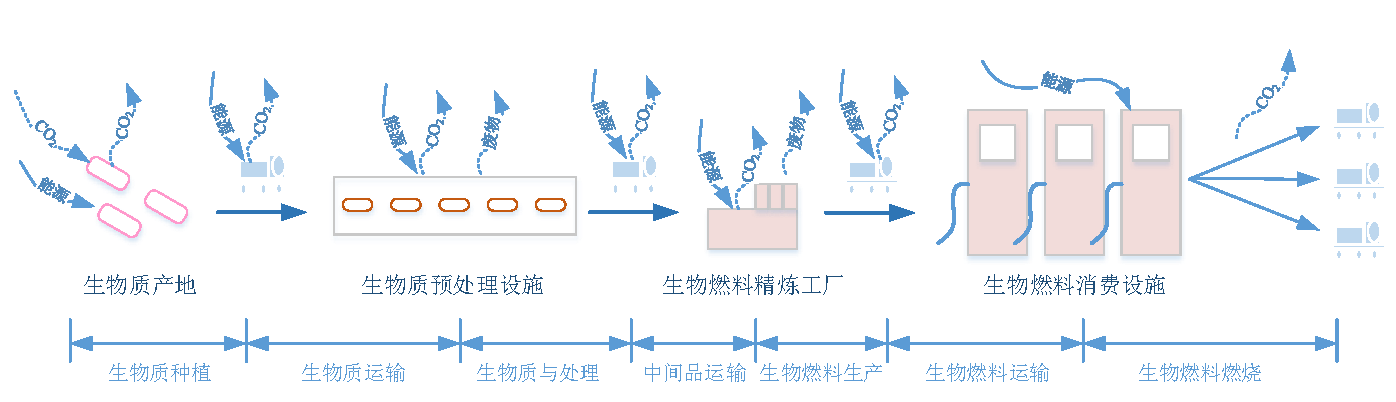
\includegraphics[width=\linewidth]{biofuelco2.pdf}
	\caption{生物燃料全生命周期各个阶段的能源消耗与碳排放示意图}
	\label{fig:biofuelco2}
\end{figure}

\subsubsection{供应链碳排放总量及其影响}
供应链碳排放总量是当前研究中评估生物燃料产业的环境影响的最重要指标。碳排放的估算方法包括排放系数法、直接监测法以及质量平衡法等。直接监测法和质量平衡法适用于微观系统,如家庭、个人行为或单个企业的单个产品的碳排放计算,因而供应链碳排放估算一般采用排放系数法,即计算各个阶段内单位输出或进程的碳排放量与 输出或进程数量的乘积\cite{Liu2014}\cite{魏巧云2014}见单位输出或进程的碳排放量估算一般有两种思路,1)归因(或追溯)法:旨在评估生物燃料系统的各个子系统中,与环境效益相关的物质流动和。因此,归因法一般采用平均数据。该方法的技术体系相对成熟,在生物燃料供应链的环境效益评估中得到广泛的应用;2)后果(或预期)法:旨在评估与化石燃料相比,生物燃料全生命周期各个阶段内的物质流向是否向环保的方向发展。因此,后果法一般采用边际排放数据。该方法的技术体系还不是十分成熟,因而应用相对较少\cite{Malca2011}。

供应链碳排放总量不仅可以直接作为生物燃料供应链环境效益的衡量指标,而且可以结合碳排放交易机制和碳税机制,从而与经济效益挂钩。《联合国气候变化框架公约的京都议定书》中将碳排放机制规定为清洁发展机制、排放交易机制和联合履行机制\cite{Hepburn2007}。其中,碳排放交易机制(又称为限额交易机制)的应用最为普遍。一方面, 该机制给予企业一定的碳排放免费配额(一般采用在一定技术水平下,生物燃料与化石燃料供应链的碳排放差额进行衡屋);另一方面,该机制允许不同企业在碳排放交易市场内开展碳排放配额的买卖,当企业的碳排放量大千免费配额时,企业需要购入碳排放配额,从而产生成本;反之,企业可以售出碳排放配额, 从而取得收入\cite{Giarola2012}碳税机制则是通过税收手段将企业产生的碳排放量转化为经济成本,它的本质是对企业的每单位碳排放进行征税。值得注意的是,一般假设仅在供应链盈利时才征收碳税,反之则不征收碳税\cite{Zamboni2011}。

碳排放量的概念是在减缓全球气候变暖趋势的背景下提出的,但是全球气候变暖仅仅是碳排放量增加的一种危害。因此为了全面地评估碳排放对生态环境造成的影响,还可以进一步结合生态环境指标体系(如Eco-indicator 99)\cite{Sabio2012},进而评估碳排放对臭氧层的破坏、对人体健康的影响、对化石燃料的损害、对矿物质的损害以及对富营养化的影响等等。

除此之外,副产品碳排放的估算是生物燃料供应链碳排放估算的另一重要内容,包括两种方法\cite{Malca2011}:1)分配法:按照主、副产品之间的某种关系(如产品价格、能星关系、物料关系等)分配碳排放星。该方法相对简单,但容易受到市场价格波动等因素影响,具有较大的随意性;2)替代法:通过扩大产品的系统边界,模拟现实中副产品的可能流向,从而分析相应的碳排放量。该方法更为贴合现实,也更具有合理性。

\subsubsection{供应链资源消耗总量}
无论是生物质种植阶段,还是燃料生产阶段,或是物流阶段,都需要消耗大量的资源(如能源、士地资源、水资源等)。因此,供应链资源消耗总童也是环境效益评估的重要内容之一。与碳排放的估算方法类似,能源\cite{Liu2014}、水资源\cite{Gerbens-Leenes2012}的消耗量估算也是基千生命周期的阶段划分,即通过单位输出或进程的资源消耗噩与输出或进程数量的乘积进行估算。生物燃料供应链的产品展千能源,因而决策者也可以采用供应链能源增加值作为衡量指标。其中, 供应链能源增加值指产出的生物燃料能值与消耗的能源能值之差。

\subsection{生物燃料供应链社会可持续性衡量方法}
与经济、环境可持续性的衡量指标相比,社会可持续性指标的计算涉及的因素更多,  更为复杂,目前尚缺乏方便、有效的衡里方法。就当前的研究文献而言,大部分文献倾向于结合模糊数学理论、多指标决策方法等数学方法,统一对经济、环境和社会可持续指标进行分析\cite{Markevicius2010, Zonin2014};另一部分文献则倾向千采用调查\cite{Oladosu2013}、仿真\cite{Affuso2013},案例分\cite{Kristoufek2012}等手段,分析生物燃料产业对土地利用、水资源利用的影响。

但是,上述方法无法直接应用于供应链优化建模之中。因此,本文针对以废弃物生 产生物燃料供应链的典型特性,倾向千选择最小化未利用的废弃物,作为社会可持续性的衡量指标之一\cite{Balaman2014}。该指标认为农场废弃物和城市餐厨垃圾的随意丢弃与处置,将对人们生活、健康造成一定的危害。因此合理地利用废弃物是一种“变废为宝”的表现,也是实现社会可持续性的一个方面。在供应链优化中,未利用的废弃物数量一般通过供应链中未被收集并且被转化的生物质数量进行衡量。


\section{生物燃料供应的不确定性}
\subsection{生物燃料供应链不确定性表现形式及其来源}
不确定性不仅是现代企业发展过程中最具挑战性的一个方面向,也是生物燃料产业发展的一个重要瓶颈问题\cite{Kim2011}。因此,供应链优化中需要充分考虑生物质供给、生物燃料需求、供应链成本、生物燃料价格等不确定性,即将不完整、不准确和/或不确定的参数值纳入建模方法之中,从而更为真实地反映供应链系统\cite{Balaman2014}。生物燃料供应链同样承受着来自方方面面的不确定性,而在供应链优化建模中忽略不确定性将产生不是最优的甚至不可行的解决方案\cite{Shabani2014}。因此,不确定条件下的生物燃料供应链优化已经成为当前研究的热点之一。

\tblref{tbl:bibliography}列举了近年来关于生物燃料供应链不确定性研究的代表性文献。大部分文献集中于解决1-2种不确定条件下的供应链优化问题,而Awudu和Zhang\cite{Awudu2012},Jiang等\cite{Jiang2014}对生物燃料供应链涉及的不确定性进行了较好的总结。Awudu和Zhang\cite{Awudu2012}将生物燃料供应链的不确定性分为生物质供给不确定性、物流不确定性、生物燃料生产不确定性、生物燃料需求与价格不确定性以及其他不确定性五类。Jiang等\cite{Jiang2014}通过对中国区域内以废弃食用油为原料的生物柴油供应链进行分析,提炼出生物质收集、生物燃料生产、生物燃料销售、生物质和生物燃料的物流以及政府与行业监管等五个环节的不确定性。

\begin{table}[htbp]
	\centering
	\zihao{5}
	\caption{生物燃料不确定性分析的代表性文献}\label{tbl:bibliography}
	\begin{tabular}{cl}
		\toprule
		主要不确定性 & \multicolumn{1}{c}{代表性文献}\\
		\midrule
		原料供给 & \cite{Awudu2012}\cite{Chen2012}\cite{Kim2011}\cite{Foo2013}\cite{Awudu2013}\cite{Shabani2014}\cite{Osmani2013,Li2014}\cite{Tong2014,Yeh2015,Tong2014a} \\
		原料价格 & \cite{Awudu2013}\cite{Giarola2012}\cite{Osmani2013}\\
		燃料需求 & \cite{Awudu2012}\cite{Kim2011}\cite{Awudu2013}\cite{Azadeh2014}\cite{Osmani2013}\cite{Tong2014,Yeh2015,Tong2014a}\\
		燃料价格 & \cite{Awudu2012}\cite{Chen2012}\cite{Kim2011}\cite{Zheng2012,Awudu2013,Azadeh2014,Giarola2012}\cite{Osmani2013}\cite{Li2014}\cite{Yeh2015}\\
		生产成本与技术 & \cite{Awudu2012}\cite{Kim2011}\cite{Li2014}\cite{Tong2014,Yeh2015} \\
		\multirow{5}{*}{其他方面} & 物流环节、政府与行业监管\cite{Awudu2012}\\
		&碳排放交易市场\cite{Giarola2012} \\
		&燃料质量\cite{Zheng2012} \\
		&设施建设成本\cite{Tong2014} \\
		&生物质种植的成本\cite{Balaman2014} \\
		\bottomrule
	\end{tabular}
\end{table}

本文在充分结合现有文献研究和生物燃料供应链运作实际的基础上,从生物质供应商、生物燃料生产商和生物燃料需求主体三个主体出发,重点分析生物质采购、生物燃料生产、生物燃料销售、物流以及政府与行业监管等五个环节的不确定性,结果如\figref{fig:uncertainty}所示。

(1)生物质采购环节的不确定性

该环节涉及的不确定性主要包括生物质数量、生物质价格、生物质类型、生物质质量以及生物质收集地点等的不确定性。生物质数量不确定性是采购环节最为重要的不确 定因素之一。对千农业废弃物而言,一方面,生物质依赖于种植、收获等作业,需要相对固定的成长周期,因此生物质的供应呈现明显的季节性特征。另一方面,在农户种植意愿、天气条件(特别是极端天气条件的发生频率、持续时间、强度等)、土壤条件等因素的共同作用下,不同种植或收获时段、不同地点的生物质产量也呈现一定的差异性\cite{Langholtz2014}。而对于废弃食用油等城市垃圾而言,一方面,生物质产量取决于城市居民的餐饮消费习惯、经济发展情况等,存在着时空差异性;另一方面,精炼工厂实际能收集到的生物质数量还受到“地沟油“非法生产产业链的竞争,从而进一步加剧了生物质数量的不确定性。

\begin{figure}
	\centering
	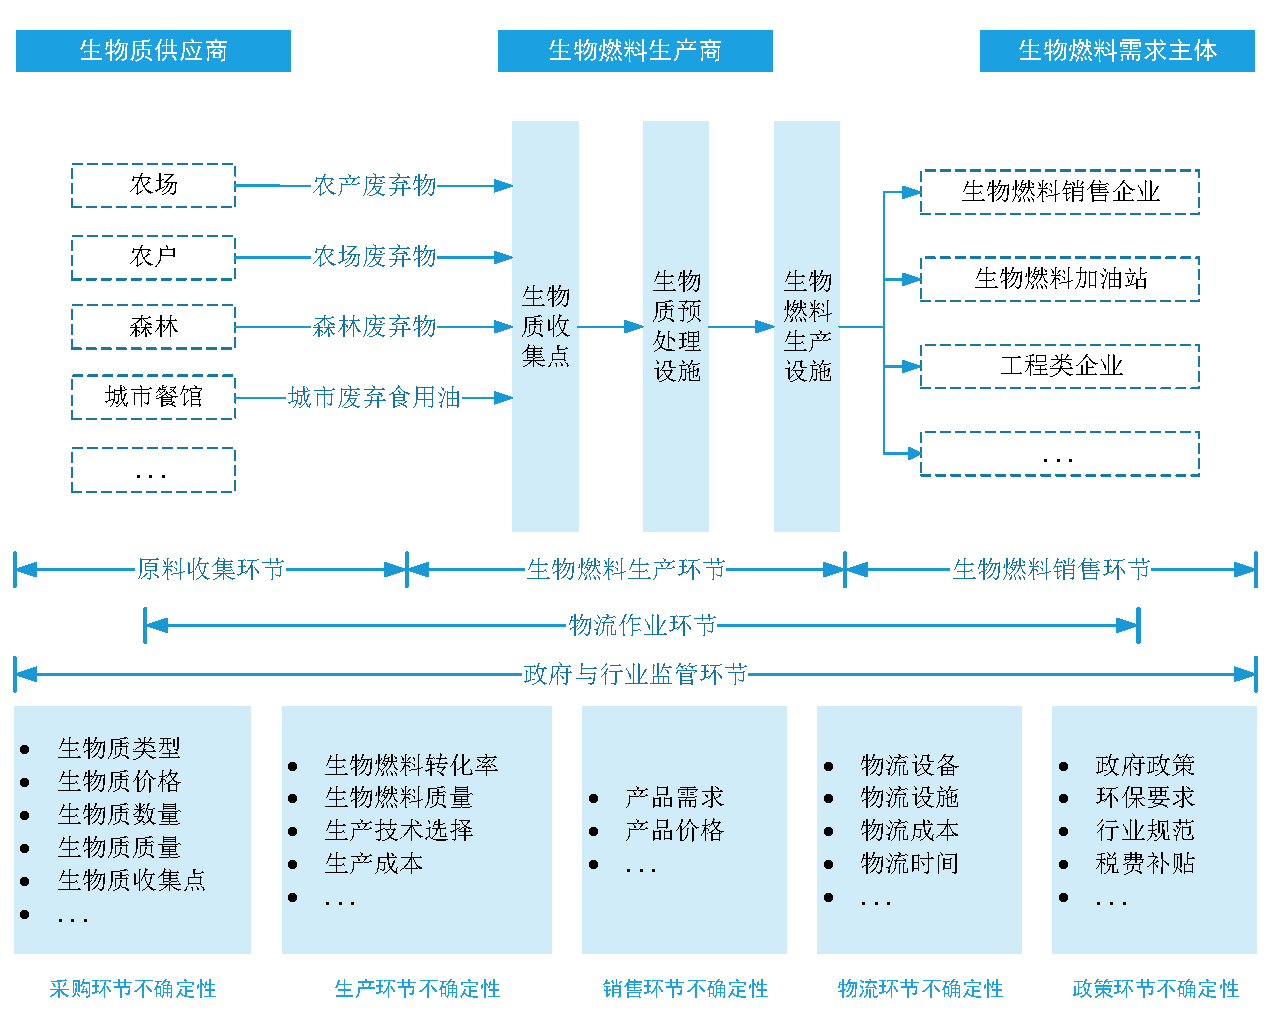
\includegraphics[width=\linewidth]{uncertainty.pdf}
	\caption{生物燃料供应链不确定性示意图}
	\label{fig:uncertainty}
\end{figure}

生物质价格不确定性是采购环节中讨论较多的另一类不确定因素。从价格的本质上看,价格不确定性是生物质市场供给和需求的市场调控结果。一方面,生物质供给水平取决于生物质产量(自身具有不确定性)\cite{Langholtz2014}; 另一方面,生物质需求水平取决于终端市场的生物燃料需求(受政府政策、居民的生物燃料接受程度等影响,具有一定的不确定性)。因此,在上述两类不确定因素的共同作用下,生物质价格表现出较大的不确定性。其他几类不确定性在生物燃料供应链优化中涉及的相对较少,但也是不可忽视的存在。生物质类型不确定性来源千农户在种植阶段的原料选择决策, 进而影响各种原料的可得性\cite{Seay2014}。农户往往综合考虑当前各种生物质的市场行惜、当地种植条件、自身种植技术以及政府政策支持等因素,确定是否种植生物质和种植的生物质类型。从国家、省等宏观层面上看, 区域的生物质种植情况(是否种植、种植类型)将在不同时间周期内呈现出一定的变化,进而对精炼工厂能收集到的生物质类型产生影响。而且在上述因素的作用下,区域的生物质可得性也存在一定的变化,从而对精炼工厂的生物质收集地点产生影响, 进而表现为收集地点的不确定性。

生物质质量不确定性指生物质中可用于转化为生物燃料的成分的含量波动,一般通过含水昼、沙石等杂质含量等指标进行衡量。对于农业废弃物而言,生物质质鱼不确定性主要受生长条件、收获技术以及农户作业的精细程度等因素影响。而对于废弃食用油等城市垃圾而言,生物质质量不确定性主要受城市饮食习惯、餐饮企业烹任习惯以及收集方式(如餐厨垃圾收集之前是否排除一定的水量)等因素影响 。

(2)物燃料生产环节的不确定性

该环节涉及的不确定性主要包括生产技术和生产绩效(如生产成本、环境影响\cite{Hammond2008}、产品产昼、产品质噩等)不确定性。生物燃料产业得到了世界各国的高度重视,而生产技术也时刻发生着变革。因此,生产技术不确定性来源千生产技术的改进或者新技术的出现\cite{Seay2014},并对生产绩效造成不可忽视的影响\cite{Gude2013}。生产绩效不仅与生产技术密切相关,而且受到工厂采用的原料类型、原料质量、库存策略以及生产策略(多原料或单原料生产) 等因素影响。此外,机器故障、员工罢工等不确定事件也会对生产计划造成影响,进而在一定程度上导致生产绩效指标的不确定性。

(3)	生物燃料销售环节的不确定性

该环节涉及的不确定性主要包括生物燃料需求、生物燃料价格、生物燃料质量、生物燃料类型等不确定性。生物燃料需求不确定性可以从两方面进行理解:一方面,生物燃料作为汽油、柴油等化石燃料的替代品之一,其需求必然取决于化石燃料的需求。而化石燃料需求又与经济发展情况、车辆拥有数量以及居民出行特性等因素相关;另一方面,与化石燃料相比,生物燃料在燃烧性能、产品价格等方面还没有被公众完全认同,因而生物燃料实际能替代的化石燃料比例成为一个极大的不确定因素。而这一比例又取 决千社会对生物燃料的接受程度、政府强制添加生物燃料的比例(如B5、E10等)等。类似地生物燃料价格基本与汽油、柴油等价格保持一致。而在当前油价大起大落的趋势下,生物燃料价格也面临着极大的不确定性\cite{Seay2014}\cite{Langholtz2014}。

对于生物燃料类型不确定性而言,在当前生产技术持续革新的背景下,生物燃料已经形成了生物柴油、生物乙醇、沼气等多种产品,加之生物燃料与化石燃料的混合比例不一的影响,其类型呈现出相当的不确定性。此外,中国生物燃料生产企业的层次参差不齐(小作坊、大企业并存的局面),采用的生产技术和设施设备也都存在较大的差异性,从而导致产出的生物燃料质量也存在较大的差别。

(4)	物流环节的不确定性

该坏节涉及的不确定性指无法将生物质和生物燃料以准时、低成本的方式送达,而导致的成本、时间等效益的差异性。物流不确定性的主要来源包括:城市交通状况、物流设备多样性(型号、容积等)、应急事件导致的交通网络中断(道路、多式联运设施等的损坏)、生物燃料工厂以及配套公用设施和资源(如电、水等)的损坏\cite{Langholtz2014} 、员工绩效水平以及供应链伙伴的协作能力\cite{Jiang2014}等。

(5)	政府与行业监管环节的不确定性

生物燃料产业尚处千发展阶段,而供应链的经营、生产等活动都离不开政府的政策支待,也时刻接受着政府和行业的监督与管理。该环节涉及的不确定性主要来源千政府与行业管理者的决策变化,进而引起的产业发展环境不确定性,具体包括:政府税收\cite{Rozakis2005}、政府补贴、鼓励性政策、生物燃料行业与相关行业的管理规范、宏观战略引出的相关发展需求(经济发展、食品安全、环境保护等)以及相关产业链的竞争(食品产业链、农产品产业链、石油产业链、地沟油非法生产产业链等)等不确定性。

\subsection{生物燃料供应链不确定性衡量方法}
不确定性的衡量指将供应链的不确定性通过数学表达式进行阐述。这不仅是现实与模型不确定性的联系桥梁,也是不确定条件下供应链优化的关键步骤之一。如何合理地表达供应链不确定性,对供应链绩效、鲁棒性等都有着不可忽视的影响。而且采用不同的方式衡量不确定性,也在一定程度上决定了后续的建模方法。就目前而言,不确定性较为成熟的衡昼方法包括清景分析法、区间刻画法、随机函数法以及模糊数法等。

(1)情景分析法

情景分析法指通过假想分析对象未来发展中可能出现的各类情景,并分析各类情景导致的相应后果。情景分析法一般有两种应用思路\cite{Chen2012}:1)“等待和检查策略”(wait-and-see approach)模拟各种随机情景的发生,并依次作出各类情景中的相应决策。该思路得出的结果在某个清景内可能表现良好,也可能造成极坏的结果(代价十分昂贵,甚至不可行)。2)“期望值策略”(expected-value solution)通过不确定参数的期望值,将各类清景整合为单一的确定情景,从而将不确定问题转化为确定性问题进行求解。这种思路相对简单,但可能产生不可靠的解决方案。在具体的应用中,情景分析法可以指定各类情景出现的概率(如随机规划),也可以不指定,仅认为存在这些情景(如鲁棒优化)。

(2)区间刻画法

在情景分析法中,分析对象可能涉及的不确定参数被限定在有限个情景之内。而在实际情况中,分析对象的可能数值不再是有限个数,而是集中于一个或若干个区间内。此时如果应用情景分析法,就必须将区间切割为有限个子区间,并以子区间作为分析单元\cite{Osmani2014}, 而这必然无法完全真实地反映不确定性。区间刻画法则适用于这一情况,它通过指定一个或多个区间的上下限以刻画不确定性,如$[100,300]$、$[100,150]\cup[200,250]$、期望值的 90\%到 110\%之间\cite{Balaman2014}等。

(3)随机函数法

随机函数法与情景分析法、区间刻画法的最大不同之处在千,分析对象的可能数值呈现为一些常见的数学函数,如正态分布\cite{Osmani2014}、均匀分布、泊松分布等。这些分布既可以从历史数据拟合中得到\cite{Giarola2012}, 也可以从不确定参数与其他不确定参数的关系中推导得到。采用随机函数法描述不确定性,不仅可以在后续的模型优化中应用已知的分布函数规律,而且可以应用蒙特卡洛仿真方法,从而大大地降低了模型的求解难度。

(4)	模糊数法

模糊数法适用于描述一些不存在明显分隔界限的对象,通过引入隶属度的概念,对分析对象属于某一类别的程度进行描述。当前研究中应用最为广泛的模糊数是三角模糊数,如$(a,b,c)$。其中,$a$,$b$,$c$,表示分析对象的可能数值由小到大的排序结果,而隶属度则由$[0,1]$区间数进行描述。当分析对象对某一类别的隶属度越大,则表示分析对象属于该类的程度越高,反之亦然。特别地,当隶属度为1时,则表示分析对象完全属于该类;而当隶属度为0时,则表示分析对象完全不属于该类。当采用模糊数法描述不确定性时,可以进一步结合模糊数学理论,从而将不确定问题转化为模糊优化问题进行求解。

\section{生物燃料供应链的鲁棒性}
\subsection{生物燃料供应链鲁棒性内涵}
一个鲁棒的供应链对千将具有竞争力的生物燃料运送到最终用户市场至关重要\cite{Awudu2012}。在未来生物燃料有可能继续扩大生产的趋势下,对生物燃料产业开展鲁棒管理是保障区域能源安全和环境效益的重要内容\cite{Langholtz2014}。目前单独地针对生物燃料供应链开展鲁棒优化研究的文献还相对较少,但一部分文献已经对电子、化工、生物等行业开展了较为深入的鲁棒优化研究,为生物质燃料供应链的鲁棒性内涵界定提供了良好的借鉴。

一般来说,鲁棒性是系统在面临内部结构和外部环境变化时,仍然能保持其系统功能的能力\cite{deng2009}。供应链作为一个复杂系统,其鲁棒性可以表述为供应链系统能够抵抗各种故障及风险,依然能够保持自身的基本结构和运作过程,从而能保证供应链的整体收益不发生较大偏差和维持持续性运行功能的能力\cite{唐莉莉2011}。生物燃料供应链的不确定性不仅来源千行业自身的内部运作,而且与农产品供应链、石油供应链等外部风险密切相关,具有相当的复杂性。因此,构建鲁棒的生物燃料供应链也更具挑战性。具体而言,生物燃料供应链的各棒性包括以下几点内涵:

1)生物燃料供应链的鲁棒性是相对的,即供应链在某种不确定条件下(如需求不确定条件)是鲁棒的,而在另一种不确定条件下(如供给不确定条件)可能是非鲁棒的。因此,供应链优化中往往只确保关键的一种或若干种不确定条件下的供应链鲁棒性。

2)生物燃料供应链的鲁棒性既不是单纯地追求效益(如经济成本、供应链利润、环境 影响等),也不是全然不顾效益,而是对效益和不确定条件下供应链适应能力的权衡。因此,一个鲁棒的供应链往往以较小的效益损失为代价,获取系统对不确定条件的适应或反应能力。

3)	生物燃料供应链的各棒优化本质上属千风险决策。因此, 鲁棒性衡量指标的选择取决于供应链决策者,如最小遗憾值、最大化最坏情景的效益、期望值等。

\subsection{生物燃料供应链舍棒性衡量方法}
鲁棒性是对不确定条件下系统效益和适应能力的综合考量, 因而选取的鲁棒性衡量指标应该能够同时反映这两个方面。总体而言,鲁棒性指标包括遗憾值、差异值和偏好值三种基本形式,而在具体应用中这些基本形式又有着多种表达方式。本文在总结相关研究文献的基础上,提炼出供应链鲁棒性的主要衡星指标。

(1)遗憾值指标

遗憾值指某个不确定情景$s\in S$的目标函数值,与所有不确定情景集合$S$中的目标函数最优值的差距,它反映了决策者对无法获取最优效益的遗憾程度。遗憾值一般通过最小期望值和最小最大值两种方式进行衡量。前者通过最小化各种情景下的遗憾值期望$\displaystyle{\sum_{s\in S}p_s(\xi_s-\xi^*)}$,而后者则通过最小化各种情景下的最大遗憾值$\displaystyle{\max_{s\in S}p_s(\xi_s-\xi^*)}$\cite{tian2012}。其中,$p_s$为各种不确定情景$s$的概率;$\xi_s$为各种不确定情景对应的目标函数值;$\xi^*$为所有不确定情景集合$S$中对应的目标函数最优值。遗憾值指标不仅可以用于目标函数,中也可以用于约束中,如控制遗憾值相对于目标函数最优值的最大比例应小于$\alpha$,即$\displaystyle{\max_{s\in S}\frac{(\xi_s-\xi^*)}{\xi^*}\leqslant\alpha}$\cite{tian2012}。

(2)差异值指标

差异值指各类不确定情景$s\in S$对应的目标函数值之间的差异性,它反映了不确定情景下目标函数值的波动情况。为方便计算,差异值一般通过各类各种情景的目标函数值与期望值$\displaystyle{\sum_{s\in S}p_s\xi_s}$或者与确定条件下的目标函数值$\xi$的差值进行衡量。前者可以表示为$\displaystyle{\sum_{s\in S}p_s(\xi_s-\sum_{s\in S}p_s\xi_s)}$,而后者则可以表示为$\displaystyle{\sum_{s\in S}p_s(\xi_s-\xi)}$。此外,差异值还可以通过目标函数值与决策者预估的目标函数值$\lambda$的差值进行衡量,如$\displaystyle{\sum_{s\in S}p_s(\xi_s-\lambda)}$。

(3)偏好值指标

偏好值指标反映了录坏情景下保证的最优效益,包括大中取小和小中取大策略\cite{yan2008}。前者适用千目标函数值越小则效益越高的清况(如经济成本、碳排放等),追求在最坏情景下的目标函数值最小,即$\displaystyle{\min\max_{s\in S}\xi_s}$;后者适用于目标函数值越大则效益越高的情况(如供应链利润、提供的就业岗位数量等),追求在最坏情景下的目标函数值最大$\displaystyle{\max\min_{s\in S}\xi_s}$。此外,偏好值还可以表示为保证某一百分比录坏情景集合下的最优效益,如90\%情景的目标函数最优值\cite{Giarola2012}。

(4)混合指标

除上述三类基本指标之外,鲁棒性还可以通过上述指标与其他指标组成的混合指标进行表示。混合指标的构建包括期望值混合和约束违反度混合两种思路。前者通过引入期望值指标$\displaystyle{\sum_{s\in S}p_s\xi_s}$表示不确定情景下的期望效益,如$\displaystyle{\sum_{s\in S}p_s\xi_s+\lambda\sum_{s\in S}p_s(\xi_s-\sum_{s\in S}p_s\xi_s)^2}$、$\displaystyle{\sum_{s\in S}p_s\xi_s+\lambda\sum_{s\in S}p_s|\xi_s-\sum_{s\in S}p_s\xi_s|}$\cite{Mulvey1995, Yu2000};后者放松各种不确定情景下所有约束都必须满足的假设,并在违反约束时,按照违反的程度对目标函数给予一定的惩罚值,$\lambda$、$\omega$为不同目标函数项的权重,如$\displaystyle{\sum_{s\in S}p_s\xi_s+\lambda\sum_{s\in S}p_s|\xi_s-\sum_{s\in S}p_s\xi_s|}+\omega\sum_{\xi\in \Xi}p_\xi\delta_\xi$\cite{Jabbarzadeh2014}。
\cleardoublepage